% ═══════════════════════════════════════════════════════════════════
% RAG & Embedding Architecture — Intelligence RM Platform
% Oracle Private Agent Factory (PAF) + Oracle ADB 26ai
% ═══════════════════════════════════════════════════════════════════
\documentclass[12pt,a4paper]{article}

% ── Packages ──────────────────────────────────────────────────────
\usepackage[utf8]{inputenc}
\usepackage[T1]{fontenc}
\usepackage{lmodern}
\usepackage[english]{babel}
\usepackage{geometry}
\usepackage{graphicx}
\usepackage{xcolor}
\usepackage{listings}
\usepackage{booktabs}
\usepackage{longtable}
\usepackage{tabularx}
\usepackage{hyperref}
\usepackage{enumitem}
\usepackage{tikz}
\usepackage{float}
\usepackage{fancyhdr}
\usepackage{titlesec}
\usepackage{caption}
\usepackage{amsmath}
\usepackage{tcolorbox}

\usetikzlibrary{shapes.geometric, arrows.meta, positioning, fit, backgrounds}

% ── Page Layout ───────────────────────────────────────────────────
\geometry{
  left=2.5cm, right=2.5cm,
  top=2.5cm,  bottom=2.5cm
}

% ── Colors ────────────────────────────────────────────────────────
\definecolor{oracleRed}{HTML}{C74634}
\definecolor{oracleDark}{HTML}{312D2A}
\definecolor{oracleBlue}{HTML}{0572CE}
\definecolor{oracleGreen}{HTML}{4B8400}
\definecolor{codeBg}{HTML}{F5F5F5}
\definecolor{codeFrame}{HTML}{CCCCCC}
\definecolor{sectionColor}{HTML}{1A3C6E}

% ── Hyperlinks ────────────────────────────────────────────────────
\hypersetup{
  colorlinks=true,
  linkcolor=oracleBlue,
  urlcolor=oracleBlue,
  citecolor=oracleBlue,
  pdftitle={RAG \& Embedding Architecture — Intelligence RM Platform},
  pdfauthor={Intelligence RM Team},
}

% ── Section styling ───────────────────────────────────────────────
\titleformat{\section}
  {\Large\bfseries\color{sectionColor}}{\thesection}{1em}{}
\titleformat{\subsection}
  {\large\bfseries\color{sectionColor!80}}{\thesubsection}{1em}{}
\titleformat{\subsubsection}
  {\normalsize\bfseries\color{sectionColor!60}}{\thesubsubsection}{1em}{}

% ── Code Listings ─────────────────────────────────────────────────
\lstset{
  backgroundcolor=\color{codeBg},
  frame=single,
  rulecolor=\color{codeFrame},
  basicstyle=\ttfamily\small,
  keywordstyle=\color{oracleBlue}\bfseries,
  commentstyle=\color{oracleGreen}\itshape,
  stringstyle=\color{oracleRed},
  breaklines=true,
  breakatwhitespace=true,
  tabsize=2,
  showstringspaces=false,
  numbers=left,
  numberstyle=\tiny\color{gray},
  xleftmargin=1.5em,
  framexleftmargin=1.5em,
  captionpos=b,
}

% ── Info Box ──────────────────────────────────────────────────────
\newtcolorbox{infobox}[1][]{
  colback=oracleBlue!5,
  colframe=oracleBlue!60,
  fonttitle=\bfseries,
  title=#1,
  arc=2mm,
  boxrule=0.5pt,
}

\newtcolorbox{warnbox}[1][]{
  colback=oracleRed!5,
  colframe=oracleRed!60,
  fonttitle=\bfseries,
  title=#1,
  arc=2mm,
  boxrule=0.5pt,
}

% ── Header / Footer ──────────────────────────────────────────────
\pagestyle{fancy}
\fancyhf{}
\fancyhead[L]{\small\textcolor{gray}{Intelligence RM Platform}}
\fancyhead[R]{\small\textcolor{gray}{RAG \& Embedding Architecture}}
\fancyfoot[C]{\small\thepage}
\renewcommand{\headrulewidth}{0.4pt}
\renewcommand{\footrulewidth}{0pt}

% ══════════════════════════════════════════════════════════════════
\begin{document}

% ── Title Page ────────────────────────────────────────────────────
\begin{titlepage}
  \centering
  \vspace*{3cm}

  {\Huge\bfseries\color{sectionColor}
    RAG \& Embedding Architecture\\[0.3em]
  }
  {\LARGE\color{oracleDark}
    Intelligence RM Platform\\[0.5em]
  }
  {\Large\color{gray}
    Oracle Private Agent Factory (PAF)\\
    Oracle Autonomous Database 26ai\\[2em]
  }

  \rule{0.6\textwidth}{0.5pt}\\[2em]

  {\large
    \textbf{Embedding Approaches Covered:}\\[0.8em]
    \begin{tabular}{rl}
      \textcolor{oracleBlue}{\textbf{1.}} & OCI GenAI Cloud Embedding (Cohere Embed v4.0)\\[0.3em]
      \textcolor{oracleBlue}{\textbf{2.}} & Oracle ADB 26ai In-Database RAG (DBMS\_VECTOR\_CHAIN)\\[0.3em]
      \textcolor{oracleBlue}{\textbf{3.}} & On-Premise Local Embedding Model (multilingual-e5-base)\\[0.3em]
    \end{tabular}
  }

  \vfill

  {\normalsize
    \textbf{Version:} 1.0\\
    \textbf{Date:} June 2026\\
    \textbf{Classification:} Internal\\
  }
\end{titlepage}

% ── Table of Contents ─────────────────────────────────────────────
\tableofcontents
\newpage

% ══════════════════════════════════════════════════════════════════
% SECTION 1 — INTRODUCTION
% ══════════════════════════════════════════════════════════════════
\section{Introduction}

\subsection{Purpose}

This document provides a comprehensive technical reference for the Retrieval-Augmented Generation (RAG) and embedding architecture implemented in the Intelligence RM (Relationship Manager) Platform. The platform leverages Oracle Private Agent Factory (PAF) and Oracle Autonomous Database 26ai to deliver AI-powered analysis across five banking scenarios:

\begin{enumerate}[label=\arabic*.]
  \item \textbf{Maturity Reminder} — Proactive deposit/product maturity alerts
  \item \textbf{Product Recommendation} — Personalized product suggestions
  \item \textbf{Campaign Eligibility} — Targeted marketing campaign evaluation
  \item \textbf{Portfolio Alert} — Market risk and portfolio monitoring
  \item \textbf{Universal Copilot} — Free-form RM assistant with multi-source RAG
\end{enumerate}

\subsection{RAG Overview}

RAG enhances Large Language Model (LLM) responses by retrieving relevant context from enterprise knowledge bases before generation. Instead of relying solely on the LLM's training data, the system:

\begin{enumerate}[label=\arabic*.]
  \item \textbf{Embeds} documents and queries into vector representations
  \item \textbf{Retrieves} the most semantically similar documents via vector search
  \item \textbf{Augments} the LLM prompt with retrieved context
  \item \textbf{Generates} a grounded, traceable response
\end{enumerate}

\subsection{Three Embedding Approaches}

The Intelligence RM Platform supports three distinct approaches to embedding, each suited to different deployment scenarios:

\begin{table}[H]
\centering
\caption{Embedding Approach Comparison}
\label{tab:approach-comparison}
\begin{tabularx}{\textwidth}{l X X X}
\toprule
\textbf{Aspect} & \textbf{OCI GenAI Cloud} & \textbf{ADB 26ai In-Database} & \textbf{On-Premise Local} \\
\midrule
Model & Cohere Embed v4.0 & Cohere Embed v4.0 (via OCI) & multilingual-e5-base \\
Dimensions & 1536 (FLOAT32) & 1536 (FLOAT32) & 768 (FLOAT32) \\
Location & OCI Cloud API & Inside Oracle Database & PAF Server (local) \\
Latency & Network-dependent & Low (in-DB) & Very low \\
Cost & Pay-per-request & Included in ADB & No API cost \\
Air-gapped & No & Partial & Yes \\
\bottomrule
\end{tabularx}
\end{table}

% ══════════════════════════════════════════════════════════════════
% SECTION 2 — ARCHITECTURE OVERVIEW
% ══════════════════════════════════════════════════════════════════
\section{System Architecture}

\subsection{High-Level Architecture}

\begin{figure}[H]
\centering
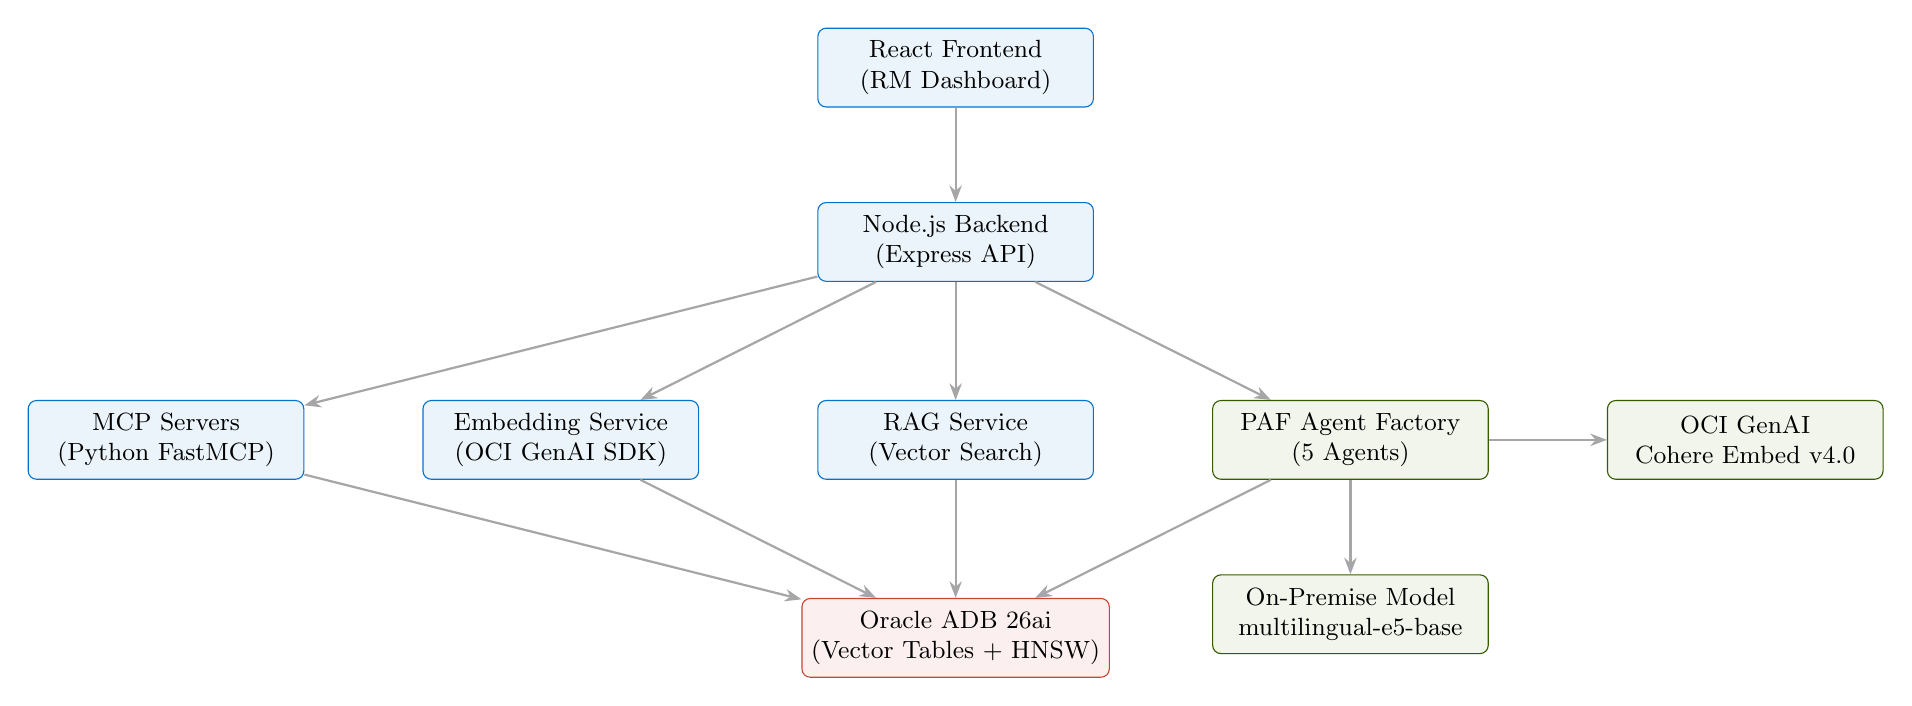
\begin{tikzpicture}[
  node distance=1.2cm and 2cm,
  box/.style={rectangle, draw=oracleBlue, fill=oracleBlue!8, minimum width=3.5cm, minimum height=1cm, align=center, font=\small, rounded corners=3pt},
  dbbox/.style={rectangle, draw=oracleRed, fill=oracleRed!8, minimum width=3.5cm, minimum height=1cm, align=center, font=\small, rounded corners=3pt},
  pafbox/.style={rectangle, draw=oracleGreen!70!black, fill=oracleGreen!8, minimum width=3.5cm, minimum height=1cm, align=center, font=\small, rounded corners=3pt},
  arrow/.style={-{Stealth[length=6pt]}, thick, color=gray!70},
]

% Row 1 — Client
\node[box] (client) {React Frontend\\(RM Dashboard)};

% Row 2 — Backend
\node[box, below=of client] (backend) {Node.js Backend\\(Express API)};

% Row 3 — Services
\node[box, below left=1.5cm and 1.5cm of backend] (embed) {Embedding Service\\(OCI GenAI SDK)};
\node[box, below=1.5cm of backend] (rag) {RAG Service\\(Vector Search)};
\node[pafbox, below right=1.5cm and 1.5cm of backend] (paf) {PAF Agent Factory\\(5 Agents)};

% Row 4 — Database
\node[dbbox, below=1.5cm of rag] (adb) {Oracle ADB 26ai\\(Vector Tables + HNSW)};

% Row 4 — External
\node[pafbox, right=1.5cm of paf] (genai) {OCI GenAI\\Cohere Embed v4.0};
\node[pafbox, below=of paf] (local) {On-Premise Model\\multilingual-e5-base};

% MCP
\node[box, left=1.5cm of embed] (mcp) {MCP Servers\\(Python FastMCP)};

% Arrows
\draw[arrow] (client) -- (backend);
\draw[arrow] (backend) -- (embed);
\draw[arrow] (backend) -- (rag);
\draw[arrow] (backend) -- (paf);
\draw[arrow] (embed) -- (adb);
\draw[arrow] (rag) -- (adb);
\draw[arrow] (paf) -- (genai);
\draw[arrow] (paf) -- (local);
\draw[arrow] (paf) -- (adb);
\draw[arrow] (mcp) -- (adb);
\draw[arrow] (backend) -- (mcp);

\end{tikzpicture}
\caption{Intelligence RM Platform — RAG Architecture Overview}
\label{fig:architecture}
\end{figure}

\subsection{Data Flow}

The RAG pipeline follows a two-phase process:

\textbf{Phase 1 — Ingestion (Offline):}
\begin{enumerate}[label=\arabic*.]
  \item Source documents (customer profiles, meeting notes, products, market data, call transcripts) are collected
  \item Text content is constructed from structured fields
  \item Embeddings are generated via one of three approaches
  \item Vectors are stored in Oracle ADB 26ai vector tables with HNSW indexes
\end{enumerate}

\textbf{Phase 2 — Retrieval (Online):}
\begin{enumerate}[label=\arabic*.]
  \item User query arrives via API or Copilot chat
  \item Query is embedded using the same model as ingestion
  \item \texttt{VECTOR\_DISTANCE()} with cosine similarity finds top-$k$ matches
  \item Retrieved chunks are injected into the LLM prompt as context
  \item LLM generates a grounded response
\end{enumerate}

% ══════════════════════════════════════════════════════════════════
% SECTION 3 — APPROACH 1: OCI GenAI Cloud Embedding
% ══════════════════════════════════════════════════════════════════
\section{Approach 1: OCI GenAI Cloud Embedding}
\label{sec:oci-genai}

This is the primary embedding approach used by the Intelligence RM Platform's Node.js backend. Embeddings are generated by calling the OCI Generative AI service via the Oracle Cloud SDK.

\subsection{Embedding Service Implementation}

The embedding service is implemented in the Node.js backend at:

\texttt{web/backend/services/embeddingService.js}

\begin{lstlisting}[language=JavaScript, caption={OCI GenAI Embedding Service (simplified)}]
const { GenerativeAiInferenceClient } = require('oci-generativeaiinference');

async function embedDocument(text) {
  const truncated = text.substring(0, 4096);
  const response = await genaiClient.embedText({
    embedTextDetails: {
      servingMode: { servingType: 'ON_DEMAND', modelId: EMBED_MODEL },
      compartmentId: COMPARTMENT_ID,
      inputs:    [truncated],
      inputType: 'SEARCH_DOCUMENT',
      truncate:  'NONE',
    }
  });
  return response.embedTextResult.embeddings[0];
}

async function embedQuery(text) {
  // Same as above but with inputType: 'SEARCH_QUERY'
}
\end{lstlisting}

\begin{infobox}[Input Types]
Cohere Embed v4.0 distinguishes between two input types:
\begin{itemize}
  \item \texttt{SEARCH\_DOCUMENT} — used when embedding documents for storage
  \item \texttt{SEARCH\_QUERY} — used when embedding user queries for retrieval
\end{itemize}
This asymmetric embedding improves retrieval accuracy by optimizing the vector space for query-document matching rather than document-document similarity.
\end{infobox}

\subsection{Configuration}

\begin{table}[H]
\centering
\caption{OCI GenAI Embedding Configuration}
\begin{tabularx}{\textwidth}{l l X}
\toprule
\textbf{Variable} & \textbf{Value} & \textbf{Description} \\
\midrule
\texttt{OCI\_GENAI\_EMBED\_MODEL} & \texttt{cohere.embed-v4.0} & Embedding model ID \\
\texttt{OCI\_GENAI\_EMBED\_DIM} & \texttt{1536} & Vector dimensions \\
\texttt{OCI\_REGION} & \texttt{us-chicago-1} & OCI region endpoint \\
\texttt{OCI\_COMPARTMENT\_ID} & (OCID) & Target compartment \\
\texttt{OCI\_TENANCY\_ID} & (OCID) & OCI tenancy \\
\texttt{OCI\_KEY\_FILE} & \texttt{./oci\_api\_key.pem} & API key PEM file \\
\bottomrule
\end{tabularx}
\end{table}

\subsection{Supported Embedding Models}

The OCI Generative AI service supports the following embedding models for RAG:

\begin{table}[H]
\centering
\caption{OCI GenAI Embedding Models}
\begin{tabularx}{\textwidth}{l c X}
\toprule
\textbf{Model ID} & \textbf{Dimensions} & \textbf{Notes} \\
\midrule
\texttt{cohere.embed-v4.0} & 1536 & Latest, highest accuracy (used in production) \\
\texttt{cohere.embed-multilingual-v3.0} & 1024 & Multilingual support (100+ languages) \\
\texttt{cohere.embed-english-v3.0} & 1024 & English-optimized \\
\texttt{cohere.embed-multilingual-light-v3.0} & 384 & Lightweight multilingual \\
\bottomrule
\end{tabularx}
\end{table}

\subsection{RAG Retrieval Implementation}

The RAG service retrieves context from multiple vector tables:

\texttt{web/backend/services/ragService.js}

\begin{lstlisting}[language=JavaScript, caption={Multi-source RAG retrieval (simplified)}]
async function retrieveForCopilot(query, customerId) {
  const vec = await embedQuery(query);
  const vecStr = `[${vec.join(',')}]`;

  // Retrieve from 4 sources in parallel
  const [profiles, notes, products, history] = await Promise.all([
    searchVectorTable('CUSTOMER_EMBEDDINGS', vecStr, 4, customerId),
    searchVectorTable('MEETING_NOTES_EMBEDDINGS', vecStr, 2, customerId),
    searchVectorTable('PRODUCT_EMBEDDINGS', vecStr, 3),
    searchVectorTable('AI_HISTORY_EMBEDDINGS', vecStr, 2, customerId),
  ]);
  return { profiles, notes, products, history };
}
\end{lstlisting}

\begin{table}[H]
\centering
\caption{RAG Source Configuration per Query}
\label{tab:rag-sources}
\begin{tabularx}{\textwidth}{l l c X}
\toprule
\textbf{Source} & \textbf{Table} & \textbf{Top-$k$} & \textbf{Content} \\
\midrule
Customer Profile & \texttt{CUSTOMER\_EMBEDDINGS} & 4 & Risk, goals, investment style \\
Meeting Notes & \texttt{MEETING\_NOTES\_EMBEDDINGS} & 2 & Historical conversations \\
Product Catalog & \texttt{PRODUCT\_EMBEDDINGS} & 3 & Product descriptions \\
AI Analysis History & \texttt{AI\_HISTORY\_EMBEDDINGS} & 2 & Prior AI insights \\
\bottomrule
\end{tabularx}
\end{table}

% ══════════════════════════════════════════════════════════════════
% SECTION 4 — APPROACH 2: Oracle ADB 26ai In-Database RAG
% ══════════════════════════════════════════════════════════════════
\section{Approach 2: Oracle ADB 26ai In-Database RAG}
\label{sec:adb-rag}

Oracle Autonomous Database 26ai provides native vector processing capabilities through \texttt{DBMS\_VECTOR\_CHAIN}, allowing embeddings to be generated and searched entirely within the database — no external application code required.

\subsection{In-Database Embedding with DBMS\_VECTOR\_CHAIN}

The embedding population scripts use PL/SQL to generate embeddings directly inside Oracle ADB:

\texttt{web/database/agent\_tools/07\_POPULATE\_EMBEDDINGS.sql}

\begin{lstlisting}[language=SQL, caption={DBMS\_VECTOR\_CHAIN embedding generation}]
DECLARE
  C_PARAMS CONSTANT VARCHAR2(500) :=
    '{"provider":"ocigenai"'
    || ',"credential_name":"OCI_GENAI_CRED_VEC"'
    || ',"url":"https://inference.generativeai.'
    || 'ap-osaka-1.oci.oraclecloud.com/'
    || '20231130/actions/embedText"'
    || ',"model":"cohere.embed-v4.0"}';
  v_content CLOB;
  v_embedding VECTOR;
BEGIN
  -- Build text from structured fields
  v_content := 'Name: ' || r.FULL_NAME
    || ' | Tier: ' || r.CUSTOMER_TIER
    || ' | Risk: ' || r.RISK_PROFILE;

  -- Generate embedding in-database
  v_embedding := DBMS_VECTOR_CHAIN.UTL_TO_EMBEDDING(
    v_content, json(C_PARAMS)
  );

  -- Store in vector table
  INSERT INTO CUSTOMER_EMBEDDINGS
    (CUSTOMER_ID, CONTENT_TEXT, EMBEDDING)
  VALUES (r.CUSTOMER_ID, v_content, v_embedding);
END;
\end{lstlisting}

\subsection{Stored Procedures for Batch Embedding}

Three stored procedures handle incremental and batch embedding:

\begin{table}[H]
\centering
\caption{Embedding Population Procedures}
\begin{tabularx}{\textwidth}{l X l}
\toprule
\textbf{Procedure} & \textbf{Source Data} & \textbf{Target Table} \\
\midrule
\texttt{EMBED\_CUSTOMER\_PROFILES} & Identity, tier, risk, income, AUM, notes & \texttt{CUSTOMER\_EMBEDDINGS} \\
\texttt{EMBED\_MEETING\_NOTES} & Summary, topics, products, follow-ups & \texttt{MEETING\_NOTES\_EMBEDDINGS} \\
\texttt{EMBED\_PRODUCT\_CATALOG} & Name, category, description, features, risk, rate & \texttt{PRODUCT\_EMBEDDINGS} \\
\bottomrule
\end{tabularx}
\end{table}

Each procedure supports two modes:
\begin{itemize}
  \item \textbf{Incremental} (\texttt{p\_mode = 'INCREMENTAL'}) — Skip rows that already have embeddings
  \item \textbf{Refresh} (\texttt{p\_mode = 'REFRESH'}) — Truncate and re-embed all rows
\end{itemize}

\subsection{OCI Credential Setup}

Database-level embedding requires OCI credentials stored as database credentials:

\texttt{web/sql/config-select-ai.sql}

\begin{lstlisting}[language=SQL, caption={OCI credential creation for in-database embedding}]
BEGIN
  DBMS_CLOUD.CREATE_CREDENTIAL(
    credential_name => 'OCI_GENAI_CRED_VEC',
    user_ocid       => 'ocid1.user.oc1..aaaa...',
    tenancy_ocid    => 'ocid1.tenancy.oc1..aaaa...',
    private_key     => '<PEM_PRIVATE_KEY>',
    fingerprint     => 'xx:xx:xx:xx:xx:xx:xx:xx'
  );
END;
\end{lstlisting}

\subsection{Vector Table Schema}

All vector tables use the \texttt{VECTOR(1536, FLOAT32)} data type with HNSW indexes:

\begin{lstlisting}[language=SQL, caption={Vector table schema example}]
CREATE TABLE CUSTOMER_EMBEDDINGS (
  ID            NUMBER GENERATED ALWAYS AS IDENTITY PRIMARY KEY,
  CUSTOMER_ID   VARCHAR2(20)  NOT NULL,
  CONTENT_TYPE  VARCHAR2(50)  DEFAULT 'profile',
  CONTENT_TEXT  CLOB,
  EMBEDDING     VECTOR(1536, FLOAT32),
  CREATED_AT    TIMESTAMP     DEFAULT SYSTIMESTAMP
);

CREATE VECTOR INDEX IDX_CUST_EMBED_VEC
  ON CUSTOMER_EMBEDDINGS (EMBEDDING)
  ORGANIZATION NEIGHBOR PARTITIONS
  WITH DISTANCE COSINE
  WITH TARGET ACCURACY 95;
\end{lstlisting}

\subsection{Vector Search with VECTOR\_DISTANCE}

Similarity search uses the native \texttt{VECTOR\_DISTANCE()} function:

\begin{lstlisting}[language=SQL, caption={Cosine similarity vector search}]
SELECT CONTENT_TEXT,
       VECTOR_DISTANCE(
         EMBEDDING,
         TO_VECTOR(:query_vec, 1536, FLOAT32),
         COSINE
       ) AS distance
FROM   CUSTOMER_EMBEDDINGS
WHERE  CUSTOMER_ID = :cust_id
ORDER BY distance ASC
FETCH FIRST 4 ROWS ONLY;
\end{lstlisting}

\subsection{Complete Vector Table Inventory}

\begin{table}[H]
\centering
\caption{Vector Tables in Oracle ADB 26ai}
\label{tab:vector-tables}
\begin{tabularx}{\textwidth}{l l X}
\toprule
\textbf{Table} & \textbf{Index} & \textbf{Purpose} \\
\midrule
\texttt{CUSTOMER\_EMBEDDINGS} & \texttt{IDX\_CUST\_EMBED\_VEC} & Customer profile vectors \\
\texttt{MEETING\_NOTES\_EMBEDDINGS} & \texttt{IDX\_NOTES\_EMBED\_VEC} & RM-customer meeting vectors \\
\texttt{PRODUCT\_EMBEDDINGS} & \texttt{IDX\_PROD\_EMBED\_VEC} & Product catalog vectors \\
\texttt{MARKET\_CONTEXT\_EMBEDDINGS} & \texttt{IDX\_MKT\_EMBED\_VEC} & Market scenario vectors \\
\texttt{AI\_HISTORY\_EMBEDDINGS} & \texttt{IDX\_AIH\_EMBED\_VEC} & Prior AI analysis vectors \\
\texttt{CALL\_CENTER\_TRANSCRIPT\_EMBEDDINGS} & \texttt{IDX\_CCT\_EMBED\_VEC} & Call transcript vectors \\
\bottomrule
\end{tabularx}
\end{table}

\subsection{PAF Agent RAG Tool Integration}

Oracle Agent Factory agents access RAG through registered database tools using \texttt{DBMS\_CLOUD\_AI\_AGENT}:

\texttt{web/database/agent\_tools/02\_TOOL\_CUSTOMER\_PROFILE\_RAG.sql}

\begin{lstlisting}[language=SQL, caption={PAF RAG tool registration}]
BEGIN
  DBMS_CLOUD_AI_AGENT.CREATE_TOOL(
    agent_name   => 'PAF_AGENT_RECOMMENDATION',
    tool_name    => 'TOOL_CUSTOMER_PROFILE_RAG',
    tool_type    => 'RAG',
    profile_name => 'DANAMON_RAG_PROFILE',
    description  => 'Retrieve customer profile context via vector similarity search'
  );
END;
\end{lstlisting}

\begin{table}[H]
\centering
\caption{PAF Agent RAG Tool Registry}
\begin{tabularx}{\textwidth}{l l X}
\toprule
\textbf{Tool Name} & \textbf{Profile} & \textbf{Description} \\
\midrule
\texttt{TOOL\_CUSTOMER\_PROFILE\_RAG} & \texttt{DANAMON\_RAG\_PROFILE} & Customer profile search \\
\texttt{TOOL\_MEETING\_NOTES\_RAG} & \texttt{DANAMON\_RAG\_PROFILE} & Meeting history search \\
\texttt{TOOL\_PRODUCT\_CATALOG\_RAG} & \texttt{DANAMON\_RAG\_PROFILE} & Product catalog search \\
\texttt{TOOL\_COPILOT\_PROFILE\_RAG} & \texttt{DANAMON\_RAG\_PROFILE} & Copilot customer search \\
\texttt{TOOL\_COPILOT\_NOTES\_RAG} & \texttt{DANAMON\_RAG\_PROFILE} & Copilot notes search \\
\texttt{TOOL\_COPILOT\_PRODUCT\_RAG} & \texttt{DANAMON\_RAG\_PROFILE} & Copilot product search \\
\bottomrule
\end{tabularx}
\end{table}

\subsection{Select AI Profiles}

Two Select AI profiles power the RAG and NL2SQL capabilities:

\begin{table}[H]
\centering
\caption{Oracle Select AI Profiles}
\begin{tabularx}{\textwidth}{l l X}
\toprule
\textbf{Profile} & \textbf{Embedding Model} & \textbf{Usage} \\
\midrule
\texttt{DANAMON\_RAG\_PROFILE} & Cohere Embed v4.0 (1536-dim) & Vector similarity RAG for all 5 agents \\
\texttt{DANAMON\_RM\_PROFILE\_GROK\_OCI} & N/A & NL2SQL on transactional tables \\
\texttt{DANAMON\_COPILOT\_PROFILE\_GROK\_OCI} & Cohere Embed v4.0 & Copilot hybrid SQL + RAG \\
\bottomrule
\end{tabularx}
\end{table}

% ══════════════════════════════════════════════════════════════════
% SECTION 5 — APPROACH 3: On-Premise Local Embedding Model
% ══════════════════════════════════════════════════════════════════
\section{Approach 3: On-Premise Local Embedding Model}
\label{sec:onprem}

Oracle Private Agent Factory (PAF) supports on-premise embedding using locally deployed models, enabling RAG in air-gapped or restricted network environments.

\subsection{Overview}

The on-premise approach runs an embedding model directly on the PAF server infrastructure, eliminating the need for external OCI GenAI API calls. This is particularly important for:

\begin{itemize}
  \item \textbf{Air-gapped deployments} — No internet connectivity required
  \item \textbf{Data sovereignty} — Sensitive text never leaves the local environment
  \item \textbf{Cost optimization} — No per-request API charges
  \item \textbf{Low latency} — Eliminates network round-trip to OCI cloud
\end{itemize}

\subsection{Supported Local Model}

\begin{table}[H]
\centering
\caption{On-Premise Embedding Model}
\begin{tabularx}{\textwidth}{l l X}
\toprule
\textbf{Model} & \textbf{Dimensions} & \textbf{Description} \\
\midrule
\texttt{multilingual-e5-base} & 768 & Microsoft's multilingual sentence embedding model, supporting 100+ languages. Pre-installed in PAF environments. \\
\bottomrule
\end{tabularx}
\end{table}

\subsection{PAF Knowledge Agent with Local Embeddings}

In Oracle Agent Factory, a Knowledge Agent can be configured to use the local embedding model through the \textbf{Model Management} screen:

\begin{enumerate}[label=\textbf{Step \arabic*:}]
  \item Navigate to \textbf{Model Management} in the PAF administration console
  \item Set \texttt{multilingual-e5-base} as the \textbf{default embedding model}
  \item Create a \textbf{Knowledge Base} with data sources (web, files, SharePoint, Google Drive)
  \item The automated pipeline processes data through: Crawling $\rightarrow$ Parsing $\rightarrow$ Storing $\rightarrow$ Chunking $\rightarrow$ \textbf{Embedding} $\rightarrow$ Ingestion
  \item Create a \textbf{Knowledge Agent} that references the knowledge base
  \item Publish and converse with the agent
\end{enumerate}

\begin{infobox}[Model Compatibility]
The default embedding model \textbf{must} be set on the Model Management screen before creating a Knowledge Agent. If an incompatible model is selected, Knowledge Agent functionality will be disabled. Both pre-built Knowledge Assistants (Oracle AI Database PAF Knowledge Assistant and Oracle Database Knowledge Assistant) are compatible with all supported embedding models.
\end{infobox}

\subsection{Data Processing Pipeline}

When using the on-premise model, the PAF automated pipeline handles the complete document lifecycle:

\begin{figure}[H]
\centering
\begin{tikzpicture}[
  node distance=0.8cm,
  step/.style={rectangle, draw=oracleGreen!70!black, fill=oracleGreen!10, minimum width=4cm, minimum height=0.8cm, align=center, font=\small, rounded corners=2pt},
  arrow/.style={-{Stealth[length=5pt]}, thick, color=gray!60},
]
\node[step] (crawl) {1. Crawling};
\node[step, below=of crawl] (parse) {2. Parsing};
\node[step, below=of parse] (store) {3. Storing};
\node[step, below=of store] (chunk) {4. Chunking};
\node[step, below=of chunk, fill=oracleBlue!15, draw=oracleBlue] (embed) {\textbf{5. Embedding} (multilingual-e5-base)};
\node[step, below=of embed] (ingest) {6. Ingestion (Vector DB)};

\draw[arrow] (crawl) -- (parse);
\draw[arrow] (parse) -- (store);
\draw[arrow] (store) -- (chunk);
\draw[arrow] (chunk) -- (embed);
\draw[arrow] (embed) -- (ingest);
\end{tikzpicture}
\caption{PAF Knowledge Agent — Document Processing Pipeline (On-Premise)}
\label{fig:pipeline}
\end{figure}

\subsection{Supported Data Sources}

PAF Knowledge Agents support multiple data source types for on-premise RAG:

\begin{itemize}
  \item \textbf{Web Sources} — Authenticated and unauthenticated web pages, including dynamic page crawling
  \item \textbf{File Uploads} — Direct document uploads (PDF, DOCX, TXT, etc.)
  \item \textbf{Microsoft SharePoint} — Enterprise document repositories
  \item \textbf{Google Drive} — Cloud document storage
  \item \textbf{File System} — Internal file system directories
\end{itemize}

\subsection{Pre-built Knowledge Assistants}

PAF ships with two pre-built Knowledge Assistants:

\subsubsection{Oracle AI Database Private Agent Factory Knowledge Assistant}
\begin{itemize}
  \item Available in non-air-gapped environments
  \item Pre-embedded with Oracle documentation using compatible models
  \item Cannot be deleted
  \item Requires wallet certificate setup if using database wallet
\end{itemize}

\subsubsection{Oracle Database Knowledge Assistant}
\begin{itemize}
  \item Installed via ``Import Dataset'' from the Datasets tab
  \item Includes Oracle product documentation, technical briefs, blogs, error messages, and feature guides
  \item Creates 5 automatic data sources during import
  \item Cannot be deleted
\end{itemize}

% ══════════════════════════════════════════════════════════════════
% SECTION 6 — MCP SERVER INTEGRATION
% ══════════════════════════════════════════════════════════════════
\section{MCP Server Integration}
\label{sec:mcp}

The MCP (Model Context Protocol) servers act as tool providers for the PAF agents, exposing database operations as callable tools.

\subsection{Architecture}

\begin{table}[H]
\centering
\caption{MCP Server Agent Ports}
\begin{tabularx}{\textwidth}{l c l X}
\toprule
\textbf{Agent} & \textbf{Port} & \textbf{File} & \textbf{Purpose} \\
\midrule
Maturity & 9011 & \texttt{agent1\_maturity.py} & Maturity reminder tools \\
Recommendation & 9012 & \texttt{agent2\_recommendation.py} & Product recommendation with RAG \\
Campaign & 9013 & \texttt{agent3\_campaign.py} & Campaign eligibility tools \\
Alert & 9014 & \texttt{agent4\_alert.py} & Portfolio alert tools \\
Copilot & 9015 & \texttt{agent5\_copilot.py} & Universal copilot tools \\
Yahoo Finance & 9016 & \texttt{agent6\_yahoo\_finance.py} & Market data tools \\
\bottomrule
\end{tabularx}
\end{table}

\subsection{MCP and Embedding}

The MCP servers (Python-based, using FastMCP) primarily serve as \textbf{tool interfaces} to the Oracle database. They do not perform embedding directly; instead:

\begin{enumerate}[label=\arabic*.]
  \item \textbf{Database tools} registered via MCP call Oracle stored procedures
  \item \textbf{Embedding generation} is handled by the database layer (\texttt{DBMS\_VECTOR\_CHAIN}) or the Node.js backend (\texttt{embeddingService.js})
  \item \textbf{RAG retrieval} leverages pre-computed vectors stored in ADB vector tables
  \item \textbf{MCP v2} uses Streamable HTTP transport (replacing SSE in v1)
\end{enumerate}

\subsection{MCP Configuration}

\begin{lstlisting}[caption={MCP Server .env configuration}]
# Oracle Autonomous Database connection
DB_USER=<db-user>
DB_PASSWORD=<db-password>
WALLET_PASSWORD=<wallet-password>
DB_DSN=irmdb_tp
WALLET_LOCATION=/path/to/wallet

# Select AI profile for NL2SQL in Copilot
SELECT_AI_PROFILE=DANAMON_COPILOT_PROFILE_GROK_OCI

# Server configuration
MCP_HOST=0.0.0.0
AGENT_MATURITY_PORT=9011
AGENT_RECOMMENDATION_PORT=9012
AGENT_CAMPAIGN_PORT=9013
AGENT_ALERT_PORT=9014
AGENT_COPILOT_PORT=9015
AGENT_YAHOO_PORT=9016
\end{lstlisting}

% ══════════════════════════════════════════════════════════════════
% SECTION 7 — VECTOR DIMENSION MIGRATION
% ══════════════════════════════════════════════════════════════════
\section{Vector Dimension Migration}
\label{sec:migration}

The platform migrated from 1024-dimensional to 1536-dimensional embeddings when upgrading to Cohere Embed v4.0.

\subsection{Migration Challenge}

Oracle Database does not support \texttt{ALTER TABLE ... MODIFY} on \texttt{VECTOR} columns (raises \texttt{ORA-51859}). The migration requires a destructive column replacement:

\texttt{web/database/agent\_tools/07b\_ALTER\_VECTOR\_DIM.sql}

\begin{lstlisting}[language=SQL, caption={Vector dimension migration procedure}]
-- 1. Drop vector indexes
DROP INDEX IDX_CUST_EMBED_VEC;

-- 2. Truncate embedding data
TRUNCATE TABLE CUSTOMER_EMBEDDINGS;

-- 3. Drop old VECTOR column
ALTER TABLE CUSTOMER_EMBEDDINGS DROP COLUMN EMBEDDING;

-- 4. Add new VECTOR column with updated dimensions
ALTER TABLE CUSTOMER_EMBEDDINGS
  ADD (EMBEDDING VECTOR(1536, FLOAT32));

-- 5. Recreate HNSW vector index
CREATE VECTOR INDEX IDX_CUST_EMBED_VEC
  ON CUSTOMER_EMBEDDINGS (EMBEDDING)
  ORGANIZATION NEIGHBOR PARTITIONS
  WITH DISTANCE COSINE
  WITH TARGET ACCURACY 95;

-- 6. Re-run embedding population
EXEC EMBED_CUSTOMER_PROFILES('REFRESH');
\end{lstlisting}

\begin{warnbox}[Destructive Operation]
This migration truncates all existing embedding data. Ensure you run the embedding population procedures in \texttt{REFRESH} mode after completing the schema migration to regenerate all vectors with the new dimensions.
\end{warnbox}

% ══════════════════════════════════════════════════════════════════
% SECTION 8 — COPILOT RAG IMPLEMENTATION
% ══════════════════════════════════════════════════════════════════
\section{Copilot RAG Implementation}
\label{sec:copilot}

The Universal Copilot is the most RAG-intensive component, combining multiple vector sources with session history recall.

\subsection{Multi-Source RAG Flow}

\begin{figure}[H]
\centering
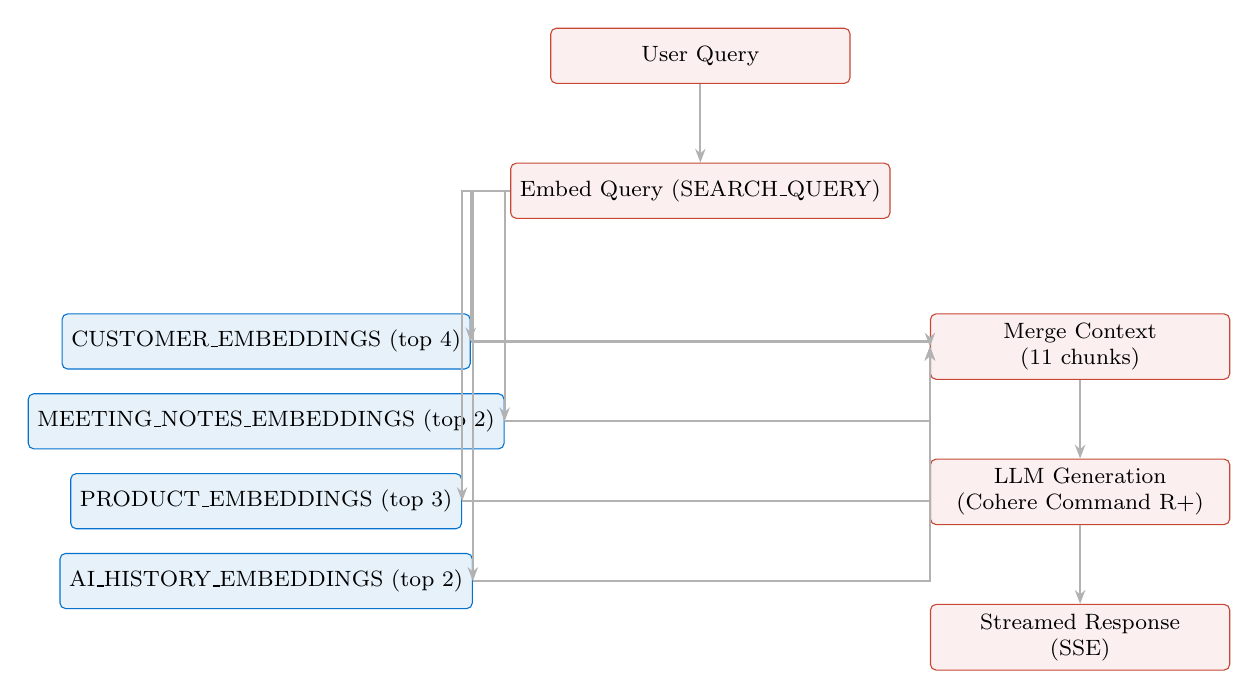
\begin{tikzpicture}[
  node distance=0.6cm and 1.5cm,
  src/.style={rectangle, draw=oracleBlue, fill=oracleBlue!10, minimum width=3.8cm, minimum height=0.7cm, align=center, font=\footnotesize, rounded corners=2pt},
  proc/.style={rectangle, draw=oracleRed, fill=oracleRed!8, minimum width=3.8cm, minimum height=0.7cm, align=center, font=\footnotesize, rounded corners=2pt},
  arrow/.style={-{Stealth[length=5pt]}, thick, color=gray!60},
]

\node[proc] (query) {User Query};
\node[proc, below=1cm of query] (embed) {Embed Query (SEARCH\_QUERY)};

\node[src, below left=1.2cm and 0.5cm of embed] (s1) {CUSTOMER\_EMBEDDINGS (top 4)};
\node[src, below=0.3cm of s1] (s2) {MEETING\_NOTES\_EMBEDDINGS (top 2)};
\node[src, below=0.3cm of s2] (s3) {PRODUCT\_EMBEDDINGS (top 3)};
\node[src, below=0.3cm of s3] (s4) {AI\_HISTORY\_EMBEDDINGS (top 2)};

\node[proc, below right=1.2cm and 0.5cm of embed] (merge) {Merge Context\\(11 chunks)};
\node[proc, below=1cm of merge] (llm) {LLM Generation\\(Cohere Command R+)};
\node[proc, below=1cm of llm] (response) {Streamed Response\\(SSE)};

\draw[arrow] (query) -- (embed);
\draw[arrow] (embed) -| (s1.east);
\draw[arrow] (embed) -| (s2.east);
\draw[arrow] (embed) -| (s3.east);
\draw[arrow] (embed) -| (s4.east);
\draw[arrow] (s1.east) -| (merge.west);
\draw[arrow] (s2.east) -| (merge.west);
\draw[arrow] (s3.east) -| (merge.west);
\draw[arrow] (s4.east) -| (merge.west);
\draw[arrow] (merge) -- (llm);
\draw[arrow] (llm) -- (response);

\end{tikzpicture}
\caption{Copilot Multi-Source RAG Flow}
\label{fig:copilot-flow}
\end{figure}

\subsection{Source Health Tracking}

The Copilot tracks RAG source availability per query, enabling graceful degradation:

\begin{lstlisting}[language=JavaScript, caption={Source health metadata emitted to client}]
// SSE event emitted to frontend
{
  type: 'sources',
  sources: {
    customerProfile: { status: 'ok', count: 4 },
    meetingNotes:    { status: 'ok', count: 2 },
    productCatalog:  { status: 'error', count: 0 },
    aiHistory:       { status: 'ok', count: 2 }
  },
  totalDocs: 8,
  failCount: 1
}
\end{lstlisting}

\subsection{AI History Embedding (Session Recall)}

Every AI analysis result is automatically embedded for future recall:

\texttt{web/backend/services/aiHistoryService.js}

\begin{lstlisting}[language=JavaScript, caption={Automatic AI history embedding}]
const content = `[${module}]\n${title}\n---\n${snippet}`;
const vec = await embedDocument(content);

await connection.execute(`
  INSERT INTO AI_HISTORY_EMBEDDINGS
    (CUSTOMER_ID, MODULE, CONTENT_TEXT, EMBEDDING)
  VALUES (:cid, :mod, :txt, TO_VECTOR(:vec, 1536, FLOAT32))
`, { cid: customerId, mod: module, txt: content, vec: vecStr });
\end{lstlisting}

% ══════════════════════════════════════════════════════════════════
% SECTION 9 — DOCUMENT CHUNKING
% ══════════════════════════════════════════════════════════════════
\section{Document Chunking Strategy}
\label{sec:chunking}

\subsection{Chunking by Source Type}

\begin{table}[H]
\centering
\caption{Chunking Strategy per Source}
\begin{tabularx}{\textwidth}{l c X}
\toprule
\textbf{Source} & \textbf{Chunked?} & \textbf{Strategy} \\
\midrule
Customer Profile & No & Single document per customer (typically $<$ 4096 chars) \\
Meeting Notes & No & Single document per meeting note \\
Product Catalog & No & Single document per product \\
Market Context & No & Single document per scenario \\
AI History & No & Single document per analysis result \\
Call Transcripts & Yes & \texttt{full\_transcript}, \texttt{summary}, \texttt{chunk\_1..N} \\
\bottomrule
\end{tabularx}
\end{table}

\subsection{Call Transcript Chunking}

For call center transcripts that exceed the 4096-character truncation limit:

\begin{itemize}
  \item \texttt{CONTENT\_TYPE = 'full\_transcript'} — Complete text (truncated at embed time)
  \item \texttt{CONTENT\_TYPE = 'summary'} — AI-generated summary
  \item \texttt{CONTENT\_TYPE = 'chunk\_N'} — Sequential text segments
  \item \texttt{CHUNK\_INDEX} tracks position (0 = full, 1+ = chunk parts)
\end{itemize}

% ══════════════════════════════════════════════════════════════════
% SECTION 10 — COMPARISON AND RECOMMENDATIONS
% ══════════════════════════════════════════════════════════════════
\section{Approach Comparison and Recommendations}
\label{sec:comparison}

\subsection{Detailed Comparison Matrix}

\begin{table}[H]
\centering
\caption{Comprehensive Embedding Approach Comparison}
\label{tab:detailed-comparison}
\begin{tabularx}{\textwidth}{l X X X}
\toprule
\textbf{Criterion} & \textbf{OCI GenAI Cloud} & \textbf{ADB 26ai In-DB} & \textbf{On-Premise Local} \\
\midrule
\textbf{Model} & Cohere Embed v4.0 & Cohere Embed v4.0 & multilingual-e5-base \\
\textbf{Dimensions} & 1536 & 1536 & 768 \\
\textbf{Invocation} & OCI SDK (Node.js) & PL/SQL (DBMS\_VECTOR\_CHAIN) & PAF internal \\
\textbf{Network} & Required (OCI API) & Required (OCI API from DB) & Not required \\
\textbf{Air-gap} & Not supported & Not supported & Fully supported \\
\textbf{Latency} & Medium (API call) & Low (in-DB, cached) & Very low (local) \\
\textbf{Cost} & Per-request & Per-request & Infrastructure only \\
\textbf{Quality} & Highest & Highest & Good \\
\textbf{Max Input} & 4096 chars & 4096 chars & 512 tokens \\
\textbf{Use Case} & Online queries & Batch population & Air-gapped RAG \\
\bottomrule
\end{tabularx}
\end{table}

\subsection{Recommended Deployment Patterns}

\begin{enumerate}[label=\textbf{\arabic*.}]
  \item \textbf{Standard Cloud Deployment:} Use OCI GenAI (Approach 1) for online query embedding and ADB In-Database (Approach 2) for batch document embedding. This is the current production configuration.

  \item \textbf{Air-Gapped / Restricted Network:} Use the on-premise local model (Approach 3) via PAF Knowledge Agent for both ingestion and retrieval. Accept the lower embedding dimensionality (768 vs 1536) in exchange for full data sovereignty.

  \item \textbf{Hybrid:} Use OCI GenAI for high-quality primary embeddings with the local model as a fallback for offline or latency-sensitive scenarios.
\end{enumerate}

% ══════════════════════════════════════════════════════════════════
% REFERENCES
% ══════════════════════════════════════════════════════════════════
\section{References}
\label{sec:references}

\begin{enumerate}[label={[\arabic*]}]
  \item Oracle Corporation, ``Create a Knowledge Agent,'' \textit{Oracle Agent Factory 25.3 Documentation}, 2025.\\
  \url{https://docs.oracle.com/en/database/oracle/agent-factory/25.3/paias/create-knowledge-agent.html}

  \item Oracle Corporation, ``DBMS\_VECTOR\_CHAIN Package,'' \textit{Oracle Database 23ai PL/SQL Packages and Types Reference}.\\
  \url{https://docs.oracle.com/en/database/oracle/oracle-database/23/arpls/dbms_vector_chain.html}

  \item Oracle Corporation, ``Oracle AI Vector Search User's Guide,'' \textit{Oracle Database 23ai}.\\
  \url{https://docs.oracle.com/en/database/oracle/oracle-database/23/vecse/}

  \item Oracle Corporation, ``OCI Generative AI — Embedding Models,'' \textit{Oracle Cloud Infrastructure Documentation}.\\
  \url{https://docs.oracle.com/en-us/iaas/Content/generative-ai/embed-models.htm}

  \item Oracle Corporation, ``DBMS\_CLOUD\_AI Package,'' \textit{Oracle Autonomous Database}.\\
  \url{https://docs.oracle.com/en/cloud/paas/autonomous-database/serverless/adbsb/dbms-cloud-ai-package.html}

  \item Oracle Corporation, ``Oracle Private Agent Factory — Model Management,'' \textit{Oracle Agent Factory 25.3 Documentation}.\\
  \url{https://docs.oracle.com/en/database/oracle/agent-factory/25.3/paias/model-management.html}

  \item Microsoft Research, ``Multilingual E5 Text Embeddings,'' \textit{Hugging Face Model Hub}.\\
  \url{https://huggingface.co/intfloat/multilingual-e5-base}

  \item Cohere, ``Embed v4 — Text Embedding Model,'' \textit{Cohere Documentation}.\\
  \url{https://docs.cohere.com/docs/embed}
\end{enumerate}

% ══════════════════════════════════════════════════════════════════
% APPENDIX
% ══════════════════════════════════════════════════════════════════
\appendix

\section{File Reference}
\label{app:files}

\begin{longtable}{p{4.5cm} p{9cm}}
\toprule
\textbf{Purpose} & \textbf{File Path} \\
\midrule
\endfirsthead
\toprule
\textbf{Purpose} & \textbf{File Path} \\
\midrule
\endhead
Embedding Service & \texttt{web/backend/services/embeddingService.js} \\
RAG Service & \texttt{web/backend/services/ragService.js} \\
OCI Configuration & \texttt{web/backend/config/oci.js} \\
Vector Table Schema & \texttt{web/backend/db/schema.sql} \\
Copilot Route & \texttt{web/backend/routes/copilot.js} \\
Embedding Population & \texttt{web/database/agent\_tools/07\_POPULATE\_EMBEDDINGS.sql} \\
Dimension Migration & \texttt{web/database/agent\_tools/07b\_ALTER\_VECTOR\_DIM.sql} \\
Customer RAG Tool & \texttt{web/database/agent\_tools/02\_TOOL\_CUSTOMER\_PROFILE\_RAG.sql} \\
Meeting Notes RAG Tool & \texttt{web/database/agent\_tools/03\_TOOL\_MEETING\_NOTES\_RAG.sql} \\
Product RAG Tool & \texttt{web/database/agent\_tools/04\_TOOL\_PRODUCT\_CATALOG\_RAG.sql} \\
Copilot RAG Tools & \texttt{web/database/agent\_tools/11\_PAF\_AGENT\_COPILOT\_TOOLS.sql} \\
AI History Service & \texttt{web/backend/services/aiHistoryService.js} \\
AI History Migration & \texttt{web/database/migrations/04\_AI\_HISTORY\_EMBEDDINGS.sql} \\
OCI Credential Config & \texttt{web/sql/config-select-ai.sql} \\
Grok Credential Config & \texttt{web/sql/config-select-ai-grok.sql} \\
MCP Server (v1) & \texttt{mcp-servers/*.py} \\
MCP Server (v2) & \texttt{mcp-servers-v2/*.py} \\
\bottomrule
\end{longtable}

\section{Environment Variables}
\label{app:env}

\begin{longtable}{p{5cm} p{3cm} p{5.5cm}}
\toprule
\textbf{Variable} & \textbf{Default} & \textbf{Description} \\
\midrule
\endfirsthead
\toprule
\textbf{Variable} & \textbf{Default} & \textbf{Description} \\
\midrule
\endhead
\texttt{OCI\_GENAI\_EMBED\_MODEL} & \texttt{cohere.embed-v4.0} & Embedding model ID \\
\texttt{OCI\_GENAI\_EMBED\_DIM} & \texttt{1536} & Vector dimensions \\
\texttt{OCI\_REGION} & \texttt{us-chicago-1} & OCI service region \\
\texttt{OCI\_COMPARTMENT\_ID} & — & Compartment OCID \\
\texttt{OCI\_TENANCY\_ID} & — & Tenancy OCID \\
\texttt{OCI\_USER\_ID} & — & User OCID \\
\texttt{OCI\_FINGERPRINT} & — & API key fingerprint \\
\texttt{OCI\_KEY\_FILE} & \texttt{./oci\_api\_key.pem} & API key PEM path \\
\texttt{DB\_USER} & — & ADB username \\
\texttt{DB\_PASSWORD} & — & ADB password \\
\texttt{DB\_CONNECT\_STRING} & \texttt{irmdb\_tp} & TNS alias \\
\texttt{DB\_WALLET\_DIR} & — & Wallet directory \\
\texttt{PAF\_ENABLED} & \texttt{true} & Enable PAF agents \\
\texttt{PAF\_BASE\_URL} & — & PAF server endpoint \\
\bottomrule
\end{longtable}

\end{document}
